\section{Introduction to the New Model}
This chapter introduces a new ``top-down'' Continuous and Proactive Security Assessment Model (CAPSAM) framework as a response to limitations in traditional risk assessment approaches. The case study by \citet{shaikh2023information} addressed the reactive nature of the Top Management Team (TMT)'s attention in its influence on the decision to carry out an Information Security Risk Assessment (ISRA). This reveals the need for a new proactive, continuous security model that integrates information security across all layers of an organisation.

\section{Overview of the CAPSAM Framework}
    \subsection{Purpose, Goals, and Intended Outcomes}
    The CAPSAM framework is designed to \textbf{address the limitations of cybersecurity models} by emphasising a proactive and continuous approach to risk assessment. Its primary purpose is to \textbf{integrate information security considerations from the earliest stages of system development} and throughout its lifecycle.

    The main goal of CAPSAM is to minimise the likelihood and impact of cybersecurity breaches through vigilant, ongoing risk management. The model aims to \textbf{integrate information security across all layers of an organisation} and focuses on continuous improvement, ensuring a resilient security posture that adapts to the ever-changing threat landscape. By doing this, CAPSAM prioritises the protection of all stakeholders\textemdash including the customer and their data\textemdash strengthening overall organisational security and trust.

    \subsection{The Five Pillars of CAPSAM}
    The core philosophies of CAPSAM can be summarised in five pillars: \textbf{Culture, Continuous, Auditing, Response, Proactive (CCARP)}. These pillars are illustrated in Figure \ref{fig:CAPSAM_Pillars} and form the foundation of the model's approach to information security risk management.

    \begin{figure}[htbp]
        \centering
        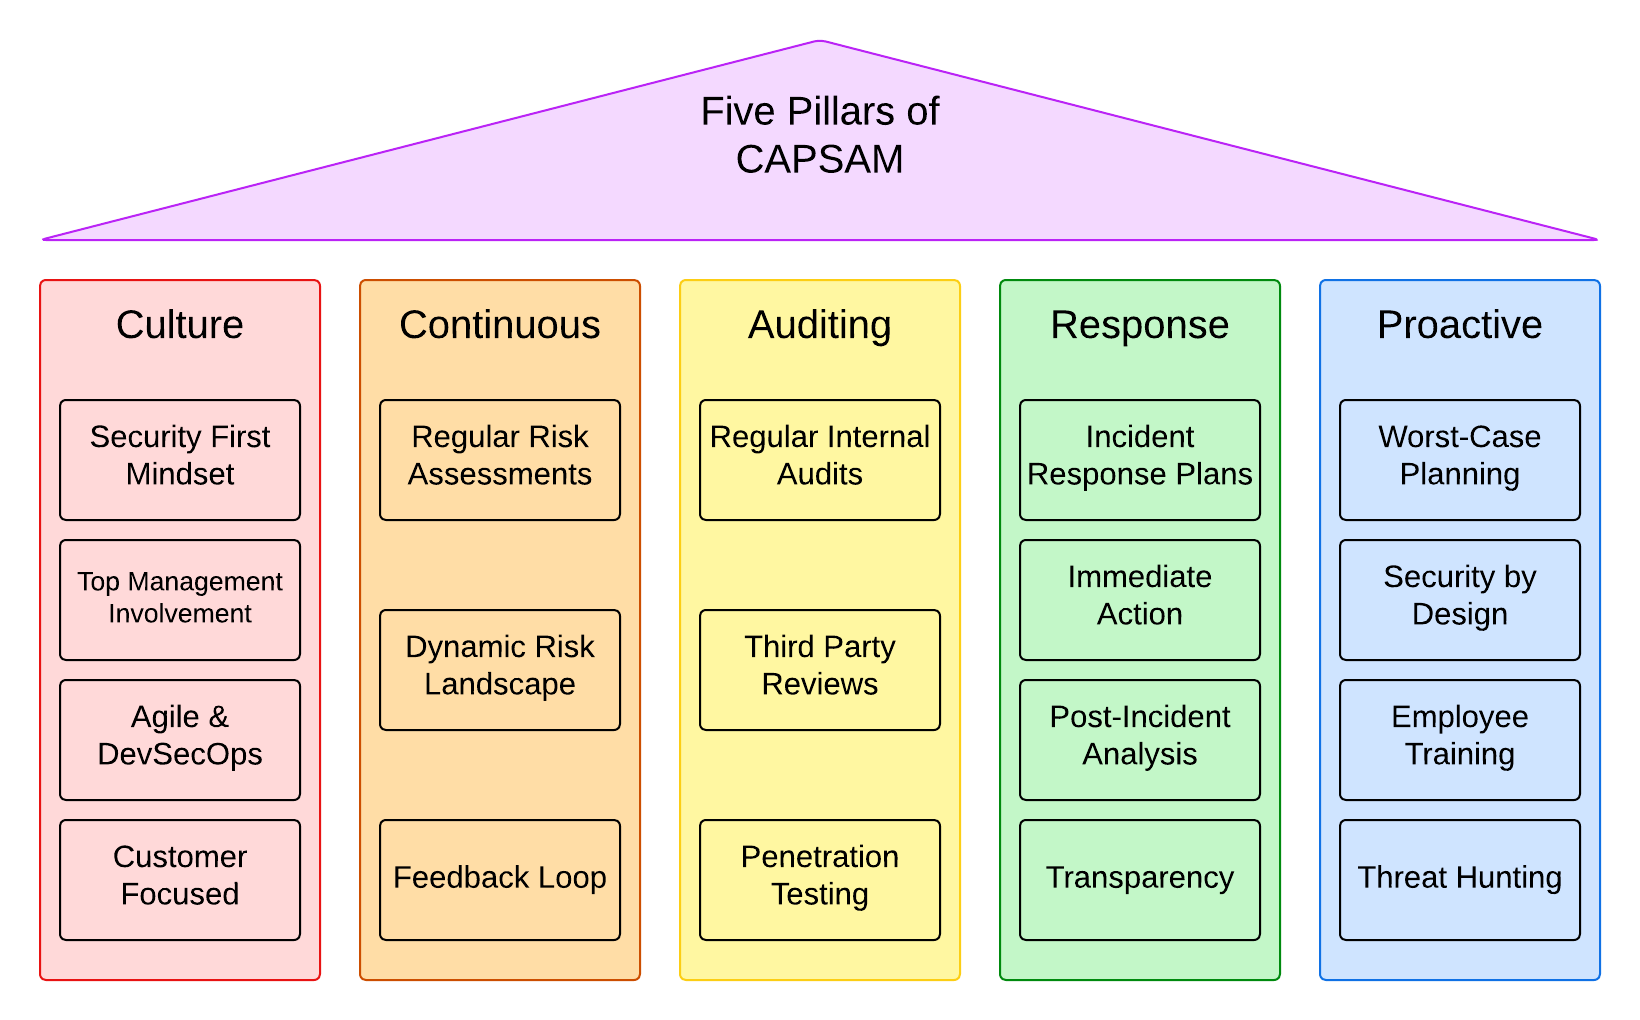
\includegraphics[width=0.8\textwidth]{figures/CAPSAM-Pillars.png}
        \caption{The Five Pillars of CAPSAM: Culture, Continuous, Auditing, Response, and Proactive (CCARP) and their components, explained in Table \ref{tab:CAPSAM_Pillars_Components} in appendices.}
        \label{fig:CAPSAM_Pillars}
    \end{figure}

    \subsection{FAMRM Cycle}
    The CAPSAM framework operates within the FAMRM cycle (New \textbf{Feature}, Information Security Risk \textbf{Assessment}, Proactive \textbf{Mitigation} Strategies, Incident \textbf{Response} Planning, and Continuous Threat \textbf{Monitoring}). This cycle ensures that each new feature or system development is subject to proactive mitigation strategies, and continuous risk assessments where feedback loops inform the next ISRA. The FAMRM cycle is illustrated in Figure \ref{fig:FAMRM_Cycle}.

    \begin{figure}[htbp]
        \centering
        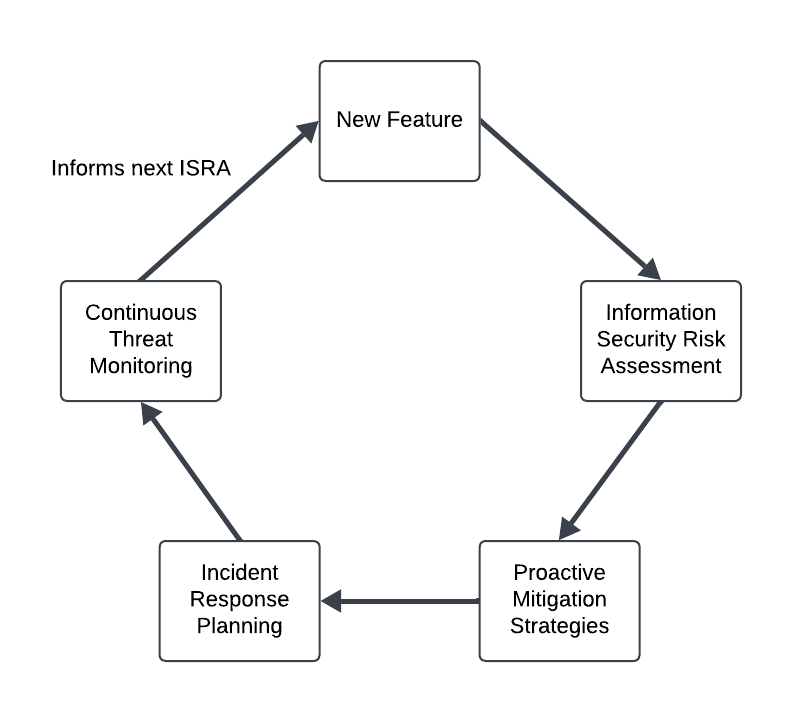
\includegraphics[width=0.6\textwidth]{figures/FAMRM-Cycle.png}
        \caption{FAMRM Cycle for Integrating Security into New Feature Development, Highlighting Continuous Risk Assessment, Proactive Mitigation, and Feedback Loops in Agile and DevSecOps Environments.}
        \label{fig:FAMRM_Cycle}
    \end{figure}

\section{Justification for a Top-Down Approach}
    \subsection{Importance of Top-Down Risk Management}
    A top-down approach to information security risk management is important for establishing a strong security posture within an organisation \citep{linkov2014risk}. It begins with executive leadership, where strategic priorities are set, resources allocated, and security policies enforced \citep{fazlida2015information}. This ensures that information security is treated as a core corporate governance issue rather than just a technical concern. In contrast, a bottom-up approach, though useful for identifying technical vulnerabilities, may lack the necessary strategic direction and executive support to address broader risks effectively \citep{linkov2014risk}.

    \subsection{Alignment with Corporate Governance}
    \citet{fazlida2015information} explain that a top-down approach aligns with corporate governance and business objectives, ensuring that the Board of Directors (BOD) and executive management recognise their responsibility to protect information assets. They elaborate that executive involvement is essential for integrating information security into the organisation's overall strategy, which is key to achieving a competitive advantage, ensuring client satisfaction, and building trust. This approach also enables the integration of security measures into daily operations, making security an essential part of all business processes.

    \subsection{Limitations of Bottom-Up Approaches}
    A primary limitation of bottom-up approaches is the lack of management buy-in, resulting in inadequate resource allocation for security initiatives \citep{fazlida2015information}. Without executive support, security may be seen as non-essential to the organisation's survival \citep{fazlida2015information}. Bottom-up strategies also struggle to coordinate efforts across departments, often focusing on technical controls while neglecting non-technical factors like human error and social engineering risks \citep{shedden2010information}. This can lead to communication breakdowns and hinder the adoption of security measures \citep{shaikh2023information}. Moreover, such approaches may overlook the complex interaction of technical, social, and economic factors that influence the organisation's risk profile \citep{cai2017cybersecurity}. A top-down approach addresses these issues by aligning policies with the organisation's needs and educating staff on the importance of information security \citep{shaikh2023information}.

\section{Theoretical Foundations}
    \subsection{Attention-Based View (ABV)}
    The Attention-Based View (ABV) theory posits that individuals have a limited capacity for attention, especially for non-routine activities \citep{shaikh2023information}. Attention is allocated based on issue salience and contextual relevance \citep{shaikh2023information}. CAPSAM applies ABV by ensuring information security remains a continuous and proactive focus, rather than a periodic or reactive task, aligning with the principle of focus of attention within ABV. By integrating security considerations from the earliest stages of system development and throughout its lifecycle, CAPSAM aims to identify and address potential risks before they can cause harm. This approach draws the attention of top management to cybersecurity, leading to greater resource allocation for security measures. The emphasis on top management involvement, as highlighted in the `Culture' pillar of CAPSAM, ensures that cybersecurity is prioritised. This aligns with findings that top management attention increases the likelihood of conducting an Information Security Risk Assessment (ISRA) \citep{shaikh2023information}. Conversely, a lack of focus on internal actions by management can result in vulnerabilities \citep{shaikh2023information}.
    
    \subsection{Agile Methodology and DevSecOps Principles}
    Agile methodologies and DevSecOps principles provide a framework supporting continuous integration, delivery, and security practices \citep{ibm2021devsecops,dingsoyr2012agile}. CAPSAM leverages these principles to maintain continuous feedback and improvement loops. Agile's adaptability and speed complement CAPSAM's proactive approach by enabling rapid adjustments to security measures, while DevSecOps integrates security throughout the development lifecycle \citep{ibm2021devsecops}. The agile manifesto, introduced in 2001, emphasised iterative development and adapting to changing requirements \citep{dingsoyr2012agile}. CAPSAM's `Continuous' pillar emphasises ongoing risk assessments and adaptation to the evolving threat landscape, supported by feedback loops that refine security measures continuously. DevSecOps principles, such as visibility and auditability, align with this focus, ensuring well-documented and adhered-to security controls \citep{ibm2021devsecops}. Additionally, Agile principles encourage accommodating changing requirements at any development stage, fitting the need for continuous adaptation in information security \citep{dingsoyr2012agile}.
    
    \subsection{ISO 31000: Risk Management Standard}
    ISO 31000 provides a comprehensive risk management framework, informing CAPSAM's approach to risk analysis, evaluation, and treatment \citep{purdy2010iso}. This standard emphasises communication, consultation, monitoring, and review, viewing risk management as central to organisational management processes \citep{purdy2010iso}. CAPSAM integrates these principles into its FAMRM cycle (Feature, Assessment, Mitigation, Response, Monitoring), ensuring risk management remains continuous and iterative. This contrasts with traditional methods offering static asset views \citep{shedden2010information}. ISO 31000 defines risk as the “effect of uncertainty on objectives,” a concept central to CAPSAM’s proactive risk management \citep{purdy2010iso}.
    
    \subsection{Organisational Learning and Continuous Feedback}
    CAPSAM emphasises continuous learning and feedback loops as critical for enhancing security, aligning with organisational learning principles that advocate adaptation and sustained improvement \citep{murray2003continuous}. The FAMRM cycle includes continuous threat monitoring, feeding directly into ongoing risk assessments, creating a dynamic feedback loop. This approach refines security measures based on insights from risk assessments, incident responses, and audits, moving beyond static quality management models \citep{murray2003continuous}. Regular internal audits and third-party reviews, including penetration testing, further support this iterative process, ensuring resilience against evolving threats. CAPSAM's commitment to ongoing learning aligns with the concept of a learning organisation, enhancing both internal efficiencies and external adaptability \citep{murray2003continuous}.
    
    \subsection{Customer-Focused Approach and Trust Theory}
    CAPSAM's customer-focused approach prioritises consumer data protection, embedding security at every stage of system development to build trust and align with corporate social responsibility (CSR) principles \citep{moir2001csr}. This approach reflects stakeholder theory, which asserts that organisations must consider the interests of all stakeholders, not just shareholders \citep{parmar2010stakeholder}. By engaging top management in cybersecurity and fostering a “security-first mindset,” CAPSAM enhances organisational credibility and reliability. Trust theory, as described by \citet{castelfranchi2010trust}, explains trust as an evaluation based on factors like ability, accessibility, and opportunities. CAPSAM integrates these principles, emphasising transparency during security incidents to maintain stakeholder trust. Trust is treated as relational capital, benefiting both the organisation and its stakeholders \citep{castelfranchi2010trust}.
    

\section{Critical Analysis and Justification}
    \subsection{Strengths of CAPSAM}
    Critically analyse the strengths of the CAPSAM model, such as its proactive nature, emphasis on stakeholder engagement, and its continuous improvement cycle. Use sources to support your claims on the benefits of proactive risk management.

    \subsection{Limitations of CAPSAM}
    Acknowledge the limitations and challenges of implementing CAPSAM. Discuss aspects such as the need for continuous updates to risk assessments, the resources required for ongoing monitoring, and the potential for over-reliance on specific teams or individuals.

    \subsection{Comparison with Case Study Approach}
    Compare CAPSAM with the reactive approach in the case study. Highlight how CAPSAM's proactive, top-down, and continuous nature addresses the gaps and limitations of the case study approach.

    \subsection{Challenges in Implementing CAPSAM}
    Discuss potential challenges in implementing CAPSAM, such as obtaining management support, ensuring consistent communication across departments, and managing the resources needed for continuous monitoring.

\section{Implementation of CAPSAM}
    \subsection{Phase 1: Planning and Preparation}
    Outline the first phase of implementing CAPSAM, which involves identifying key stakeholders, defining roles and responsibilities, and establishing communication channels. Discuss the importance of aligning the security risk management policy with the organisation's overall strategy.

    \subsection{Phase 2: Implementation}
    Describe the process of conducting risk assessments, identifying vulnerabilities, prioritizing risks, and developing mitigation strategies. Explain the importance of integrating risk management activities with the software development lifecycle.

    \subsection{Phase 3: Review and Improvement}
    Detail the review phase, which involves regular assessments of the CAPSAM framework, adapting the model based on insights and business changes, and fostering a culture of continuous security improvement.

\section{Conclusion}
Summarize the key points discussed in the chapter, reinforcing the value of the CAPSAM framework in overcoming the limitations of traditional risk assessment models. Emphasize the importance of a proactive, continuous approach to information security and its alignment with business practices and strategic goals.